The hypercube topology has two nodes along each dimension and $\log_2 n$ dimensions.  The construction of a hypercube goes as follows, in general a $d-$dimensional hypercube is constructed by connecting corresponding nodes of two $(d-1)$ dimensional hypercubes \Fig{hypercube_basic}.\\

\begin{figure}[!ht]
\centering
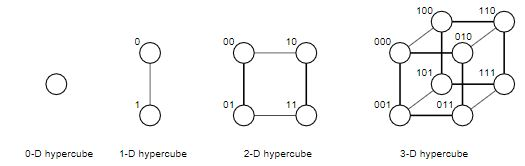
\includegraphics[width=1\columnwidth]{figure/hypercube_basic.JPG}
\caption{Hypercube in $0$, $1$, $2$, $3$ dimension. \cite{Informatik5}}
\label{fig:hypercube_basic}
\end{figure}

In this work, we have two tasks as follows :
\begin{itemize}
\item One data injection, we propose a method of finding an optimal distribution of a divisible job among a cluster of processors connected by communication links and forming a hypercube network.  The methodology we apply is similar to the flow matrix technique.\\
\item Sensitivity analysis of the hypercube structure by adding more processors or dimensions.
\item The multi-source sub-optimal algorithms to speedup job execution.
\begin{itemize}
\item The data injection fractions are even.
\item The data injection fractions are different with each other.
\end{itemize}
\end{itemize}

\subsection{Data Injection On The Grid Processor}
For the hypercube of dimension $d$ there are $2^{d}$ processor in the system.  Each of the processors has direct links to $d$ neighbors.  A method of naming the processors is to use label consisting of a binary string $d-$ position long.  Further, the label of a processor is a binary number from the interval $[0, 2^{d}-1]$

To address the qualitative model of computation, the critical problem is to calculate the number of processor on each $D_{i}$.  Each node is connected by link and the hamming distance of their's label is $1$.  According to the lemma of \cite{blazewicz1995scheduling}, \\

\begin{lemma}
In each layer $i$ of $d-$dimensional hypercube, there are ${n \choose i}$ processors each of which can be accessed through $i$ communications links and is capable of transmitting to $d-i$ still idle processors.
\end{lemma}

According to a $2-D$ hypercube \Fig{2t2}, the flow matrix is  
\begin{equation}
{
A = \left[ \begin{array}{ccc}
{2 \choose 0} & {2 \choose 1} & {2 \choose 2}\\
1 & -1 & 0\\
0 & \sigma-1 & 1
\end{array} 
\right ]
=
\left[ \begin{array}{ccc}
1 & 2 & 1\\
1 & -1 & 0\\
0 & \sigma-1 & 1
\end{array} 
\right ]
} 
\end{equation}
, which is investigated in Regular Network Chapter.\\

According to a $3-D$ hypercube, the flow matrix is \\

\begin{equation}
{
A = \left[ \begin{array}{cccc}
{3 \choose 0} & {3 \choose 1} & {3 \choose 2} & {3 \choose 3}\\
1 & -1 & 0 & 0\\
0 & \sigma-1 & 1 & 0\\
0 & \sigma-1 & \sigma & 1\\
\end{array} 
\right ]
=
\left[ \begin{array}{cccc}
1 & 2 & 2 & 1\\
1 & -1 & 0 & 0\\
0 & \sigma-1 & 1 & 0\\
0 & \sigma -1 & \sigma & 1
\end{array} 
\right ]
} 
\end{equation}
\\

The speedup is $\left | -\det A \right |$.
\newpage
A general case, $D-$dimension network, the flow matrix is :
\begin{equation*}
     {A = \left[ \begin{array}{ccccccc}
{n \choose 0} & {n \choose 1} & {n \choose 2}  & \cdots & {n \choose n-2} &{n \choose n-1} & {n \choose n} \\
1 & -1 & 0 & \cdots& 0 & 0 & 0\\
0 & \sigma-1 & 1 & \cdots & 0 & 0 & 0 \\
0 & \sigma-1 & \sigma & 1 & 0 & \cdots & 0 \\
0 & \sigma-1 & \sigma & \sigma & 1 & 0 & 0 \\
\vdots & \vdots & \vdots  &   \vdots & \ddots & \ddots\\
0 & \sigma-1 & \sigma & \cdots & \sigma & \sigma & 1
\end{array} 
\right ]}
\end{equation*}



